\begin{figure}[!h]
	\centering
	\subbottom[before adjustment\label{fig:egbfradj}]{
		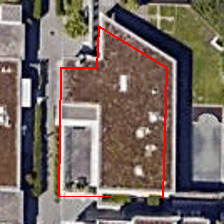
\includegraphics[width=\figfigfigfig\textwidth]{4-04-0.png}
		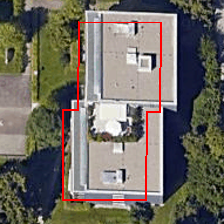
\includegraphics[width=\figfigfigfig\textwidth]{4-04-1.png}
		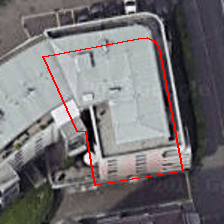
\includegraphics[width=\figfigfigfig\textwidth]{4-04-2.png}
		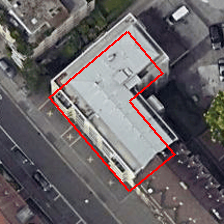
\includegraphics[width=\figfigfigfig\textwidth]{4-04-3.png}
	}
	\subbottom[after adjustment\label{fig:egaftadj}]{
		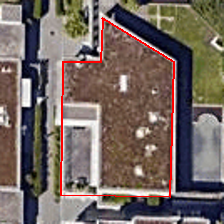
\includegraphics[width=\figfigfigfig\textwidth]{4-04-4.png}
		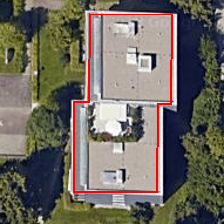
\includegraphics[width=\figfigfigfig\textwidth]{4-04-5.png}
		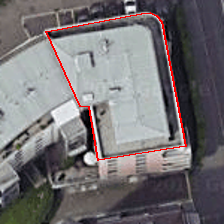
\includegraphics[width=\figfigfigfig\textwidth]{4-04-6.png}
		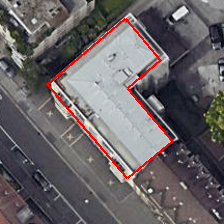
\includegraphics[width=\figfigfigfig\textwidth]{4-04-7.png}
	}
    \caption{Adjustment examples. (a) shows the polygons before adjustment, while (b) shows the polygons after adjustment.}
	\label{fig:egadj}
\end{figure}